
% Honours Report Template
% updated May 2013
%
\documentclass[a4paper,12pt]{article}
%\makeatletter
%\renewcommand\paragraph{\@startsection{paragraph}{4}{\z@}%
%{-2.5ex\@plus -1ex \@minus -.25ex}%
%{1.25ex \@plus .25ex}%
%{\normalfont\normalsize\bfseries}}
%\makeatother
%\setcounter{secnumdepth}{4} % how many sectioning levels to assign numbers to
%\setcounter{tocdepth}{4}    % how many sectioning levels to show in ToC
%
\usepackage[section]{placeins}
\usepackage{pbox}
\usepackage{epsfig}
\usepackage{latexsym}
\usepackage{graphicx}
\usepackage[square,numbers,sort&compress]{./natbib/natbib}
\usepackage{url}
\usepackage{caption}
\usepackage{subcaption}
% It also sets the bibliographystyle to plainnat; for more information on
% natbib citation styles, see the natbib documentation, a copy of which
% is archived at http://www.jmlr.org/format/natbib.pdf
\usepackage{setspace}
\usepackage{amsmath}
\usepackage{amssymb}
\usepackage{amsfonts}
\usepackage{color}

%\graphicspath{{./figures/}
%Formatting-------------------------------------------------------------------
%\renewcommand{\refname}{\textbf{Literature}}
%
\renewcommand{\contentsname}{\small\textbf{{\center Table of Contents}}}
%
\setlength{\textheight}{8.8in}
%
\setlength{\topmargin}{-1.5cm}
%
\doublespacing
%\setlength{\textwidth}{17cm}
%
%\setlength{\oddsidemargin}{-0.1714in}
%
% Boxit -----------------------------------------------------------
\setlength{\fboxrule}{0.2mm} \setlength{\fboxsep}{4mm}
%
\newsavebox{\savepar}
\newenvironment{boxit}{\begin{lrbox}{\savepar}
        \begin{minipage}[b]{4.6in}}
        {\end{minipage}\end{lrbox}\fbox{\usebox{\savepar}}}
        
        
 \hyphenation{op-tical net-works Mathe-ma-tical street-scape street-scapes aes-the-tics aes-the-tic com-pu-ting geo-metric Geo-me-tric geo-metry boun-da-ries de-ve-lop-ment know-ledge mani-fold mani-folds high-di-men-sio-nal}
%
%
%
% Document-----------------------------------------------------------------------
%
\begin{document}
%
\title{\bf Technology \& User Engagement}
%
\author{Ross Bille\\
School of Electrical Engineering \& Computer Science\\
The University of Newcastle\\ Callaghan NSW 2308, Australia\\
Email: \texttt{c3127333@uon.edu.au} } 
\maketitle


\newpage
\begin{abstract}%
\noindent Document abstract 
\end{abstract}

\pagebreak

\tableofcontents

\pagebreak

\listoffigures        

\pagebreak

\section{Introduction}
%User engagement and why we need it
Systems are created daily to achieve a set of goals, these goals vary greatly depending on the environment that the system has to run in, be it in the workplace, schools, community, or general commercial systems. Regardless of the environment, the types of systems that will be discussed in this paper all share one thing, that is to achieve their goals they all require users to interact with the system in one way or another. 
This interaction needs to be present throughout the entire life cycle of the system; however this paper will mainly discuss two phases of this life cycle, the initial implementation and continued execution of the system. 
This paper will discuss what should be present during the initial implementation of a system, in order to get users interested in interacting with the system, and what techniques we can use to keep users motivated through the continued execution of a system. In 2006~\citet[p.~1]{fun-of-use} mentions ``Successful software products should arouse positive emotions'', thus further outlining another aim of software systems in particular that when met can assist in motivation~\citep{fun-of-use}.

\subsection{The City Evolutions Project}
%introduction to city evolutions project
Newcastle City Council (NCC) were interested in increasing tourism through Newcastle and in particular through Watt Street. To do this NCC in collaboration with Newcastle Now and the University of Newcastle (UON) developed the City Evolutions Project. The main idea of this project was to promote Newcastle's rich cultural and historical aspects. 
The project required ten sites to be set up through Watt Street each containing a projector with some sites also housing a computer, a wireless hotspot, and a motion detecting camera. The aim being that material expressing the cultural and historical aspects of Newcastle was projected onto the sides of buildings between sunset and 10pm every day.\\
In order for this project to be a success the displayed content needs to interest and attract people to Watt street and also motivate them to keep coming back, thus ultimately increasing tourism. Which brings us into the reason for the research that this paper presents.

\section{Current Fields Utilising Technology for User Engagement}\label{sec:current-fields}
The following sections introduce some areas of everyday life that have implemented systems which rely on user engagement for their success. We also discuss these systems and what goals they set out to achieve.

\subsection{Workplace}

In the workplace systems have been introduced in order to share information (such as health plan offerings~\citep{taxonomy-of-gamification})  throughout the company, and increase worker productivity measured through key performance indicators (KPI's).
Some systems include (but not limited to):
\begin{itemize}
	\item{Bonus Schemes}
	\item{Online portals~\citep{taxonomy-of-gamification}}
	\item{Inter-office games~\citep{taskville}}
\end{itemize}

\subsubsection{Taskville}\label{sec:taskville}
Taskville is one such system designed to be implemented in the workplace~\citep{taskville}. Taskville was designed to ``address key challenges in contemporary distributed and diverse workplaces''~\citep[p.~4]{taskville}. 
It does this by implementing a game that is to be played by the different groups of an organisation, where each group  has a city in the game that they must grow and control. Taskville implements gamification (see section~\ref{sec:gamification}) techniques such as rewards (see section~\ref{sec:rewards}) in form of in-game currency that can be spent on buildings, and points that are used to define who is the mayor of each city, both of which can be earned by meeting KPI's or completing defined tasks.\\ Taskville was found to increase the awareness of the work performed by other groups within the workplace and at the same time encouraged each individual to outperform other group members in order to reach the title of mayor~\citep{taskville}.

\subsubsection{Agentville}\label{sec:agentville}
Agentville is a tool developed to assist employees of a call center in managing their KPI's~\citep{production-environments}. As call centers already monitor statistics such as:
\begin{itemize}
	\item{Average Handle Time (AHT)~\citep{production-environments},}
	\item{Occupancy~\citep{call-center},}
	\item{Abandoned calls~\citep{call-center},}
	\item{Calls answered~\citep{call-center},}
	\item{Calls offered~\citep{call-center},}
	\item{Average wait time~\citep{call-center}, and}
	\item{Grade of service~\citep{call-center}}
\end{itemize}
the application was not developed to create more statistics to monitor but to help each individual keep track of their own statistics in relation to the rest of the organisation~\citep{production-environments}.

\subsection{Education}\label{sec:education}
Educational institutes implements many different systems with many different aims, two such aims are: handling behavior and motivating students to learn.

\par
Advancements in technology have led to it being adopted within the educational sector~\citep{distance-education}, this has led to technologies such as the Internet and virtual reality (VR) being adopted in all forms of education~\citep{virtual-reality}.
The following sections discuss what systems have been implemented throughout a few aspects of education, from simple paper-based systems to advances VR systems.

\subsubsection{Classroom}\label{sec:classroom}
Walk into almost any primary school classroom and you will see a poster with a list of students names with stickers next to these names. This is a system that teachers use to reward students and publicly display achievements to the class, this is done to encourage competition between the students, which in turn motivates them to do better~\citep{school-kids}.

\subsubsection{Online Learning}
With the advancements in technology over the past few years universities around the world have started offering courses by distance in an online manner; in addition to this, there are many websites dedicated to teaching content to anyone that wants to learn it.

\paragraph{\indent~University Distance Education.}
Generally with higher education there is less emphasis on the initial interest of the student and more on keeping the student motivated once they have enrolled in a course, this is due to the content itself interesting the students. Unfortunately keeping students motivated after their initial interest wears off is the difficult part, this becomes more apparent when it comes to distance education~\citep{distance-education}.
Generally the students that enroll in courses online are of mature age and sometimes they have other focuses in life~\citep{distance-education}.

\par
Universities around the world have been taking steps to increase this motivation, largely through the use of multimedia, lectures can now be pre-recorded and streamed to students all around the world. Universities around the world, have adopted this technique, however this is still not enough and this paper will describe some more techniques that would be of great benefits to this type of education (see section~\ref{sec:techniques-to-enhance}).

\paragraph{\indent~Educational Websites.} 
Coursera is an online collaboration of universities such as (but not limited to): 
\begin{itemize}
	\item{Stanford University,}
	\item{Yale University,}
	\item{The University of Tokyo, and}
	\item{HEC Paris}
\end{itemize}
Coursera aims to create a collaborative environment for users to learn and teach each other. The universities that contribute to Coursera use the above mentioned technique of streaming lectures to students and users; however there are a few more techniques that are implemented in order to assist in motivating students, one of these techniques is the use of social media to share achievements which will be explained in more depth in sections~\ref{sec:gamification} and~\ref{sec:social-media}.

\par
Another educational website, Codecademy, specialises in teaching programming skills in various languages. A student is given the option to choose what they want to learn and they can set their own pace, giving the students a sense of autonomy which has been found to assist with intrinsic motivation~\citep{bread-and-games}. Codecademy also implements a few gamification techniques (see section~\ref{sec:gamification}) such as badges (which can be seen in figure~\ref{codecademy-badges}) mixed with social media aspects (see section~\ref{sec:social-media}) to keep the student coming back day after day.	

\begin{figure}[!ht]
	\centering
	\begin{minipage}{.5\textwidth}
	  \centering
	  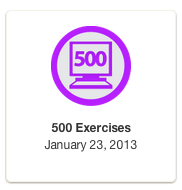
\includegraphics[width=.6\linewidth]{./images/codecademy-badge-500exercises}
	  \label{codecademy-badge-500exercises}
	\end{minipage}%
	\begin{minipage}{.5\textwidth}
	  \centering
	  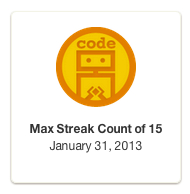
\includegraphics[width=.6\linewidth]{./images/codecademy-badge-maxstreak}
	  \label{codecademy-badge-maxstreak}
	\end{minipage}
	\caption{Codecademy badges}
	\label{codecademy-badges}
\end{figure}

\subsection{Therapy}
Researchers have recently been looking into alternate methods for delivering cognitive behavioral therapy to patients, with recent studies showing that computerised methods compare very well with the traditional face to face methods~\citep{games-for-behavior-change}. One of the reasons identified in~\citep{games-for-behavior-change} is the ``difficulty or tediousness of using the tools''~\citep[p.~2]{games-for-behavior-change}, which is one of the issues this paper aims to address (specifically see section~\ref{sec:effort-reduction}).

\subsection{Commercial}
The commercial industry utilises many different types of systems in order to sell products and keep selling products, with one of the most prominent being rewards systems. Rewards systems in the commercial industry vary from paper based frequent visit cards to digital points tracking systems. The following sections discuss some of these systems, in particular the digital renditions, and how they are achieving user engagement, as well the benefits to the business.

\subsubsection{Paper Based}
Paper based rewards cards are on their way out with most companies turning to digitally tracking a customers purchases. Regardless it is still worth mentioning these systems as they form the basis for their digital cousins.

\par
The basics of these paper based rewards are as follows, customers are given a card that gets stamped or punched every time the customer completes a task (commonly making a purchase), once the customer meets a certain requirement they are rewarded, the reward depends on the business but generally consists of a discount on the next purchase. This form of reward is referred to as an extrinsic reward, section~\ref{sec:extrinsic} will discuss this further.

\subsubsection{Digital}
Bringing the above mentioned rewards systems into the digital world allows the implementers to expose some extra techniques. One such technique being the introduction of gamification (see section~\ref{sec:gamification}), an example of this is Starbucks rewards system where \textbf{achievements} are earned, such as free refills, after \textbf{leveling up} your reward card through making purchases~\citep{gamifying-intelligent-environments} and interacting with the application that is available along side the card.

\begin{figure}[!ht]
	\centering
	\begin{minipage}{.5\textwidth}
	  \centering
	  \includegraphics[width=.6\linewidth]{./images/clubCard-boost}
	  \captionof{figure}{Boost's Club card~\citep{boost}}
	  \label{clubCard-boost}
	\end{minipage}%
	\begin{minipage}{.5\textwidth}
	  \centering
	  \includegraphics[width=.6\linewidth]{./images/clubCard-sca}
	  \captionof{figure}{Super Cheap Auto's Club+ card~\citep{sca}}
	  \label{clubCard-sca}
	\end{minipage}
\end{figure}

\par
These types of cards are used throughout many different businesses in order to track what users purchase, which ultimately benefits the business. Because using these cards is optional it can be seen that these systems must offer some way of motivating a user.

\subsection{Community}
Lately there have been many different applications being published each with the aim to modify the behavior of the general population. The following sections analyse some of these applications and discuss the methods used to increase a users interaction with the application.

\subsubsection{Nike+}


\subsubsection{I-GEAR}
I-GEAR is a project currently being run by the University of Luxembourg in order to encourage commuters to modify their transport behaviors, to ultimately reduce congestion~\citep{igear,igear-2}. Researchers on the I-GEAR project are looking into how gamification techniques can be used to make the project successful.

\subsubsection{RunKeeper}
RunKeeper is a fitness application dedicated to motivate people to get fit. RunKeeper measures and tracks its users physical activities, helping them set goals and fulfill achievements. RunKeeper pits its users againsts each other in order to utilise their natural desire to win~\citep{desire-to-win}.

\begin{figure}[!ht]
\centering
\begin{minipage}{.5\textwidth}
  \centering
  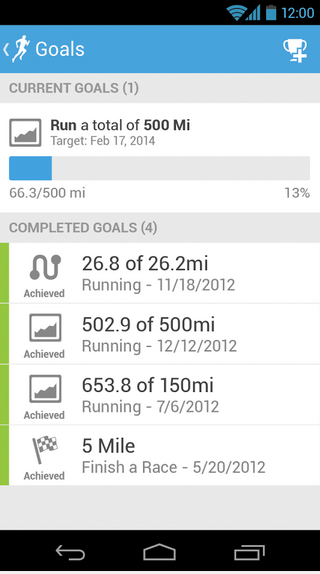
\includegraphics[width=.6\linewidth]{./images/application-runkeeper-goals}
  \captionof{figure}{RunKeeper achievements~\citep{runkeeper}}
  \label{application-runkeeper-achievements}
\end{minipage}%
\begin{minipage}{.5\textwidth}
  \centering
  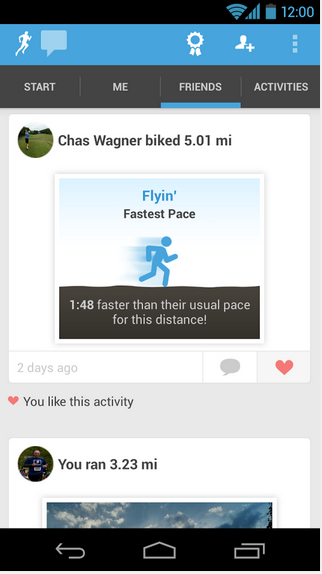
\includegraphics[width=.6\linewidth]{./images/application-runkeeper-socialnetworking}
  \captionof{figure}{RunKeeper networking~\citep{runkeeper}}
  \label{application-runkeeper-social}
\end{minipage}
\end{figure}


\subsubsection{QuitNow!}
QuitNow! is a smartphone application designed to aid its users through the process of quitting smoking.
In order to motivate its users QuitNow! tracks their success in the form of achievements, rewarding them with badges in order to ``motivate you[its users] to achieve your goal''\citep{quitnow}. QuitNow! also implements an internal social networking aspect in order to utilise our natural competitive desire~\citep{bread-and-games}.\\

\begin{figure}[!ht]
\centering
\begin{minipage}{.5\textwidth}
  \centering
  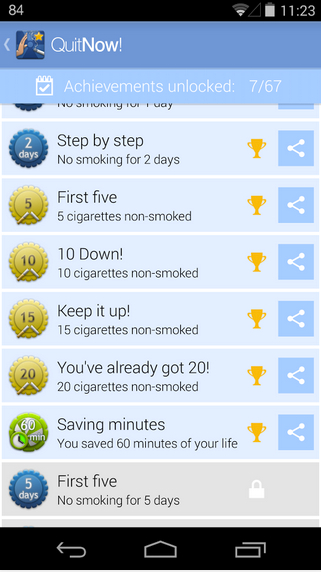
\includegraphics[width=.6\linewidth]{./images/application-quitnow-achievements}
  \captionof{figure}{QuitNow! achievements~\citep{quitnow}}
  \label{application-quitnow-achievements}
\end{minipage}%
\begin{minipage}{.5\textwidth}
  \centering
  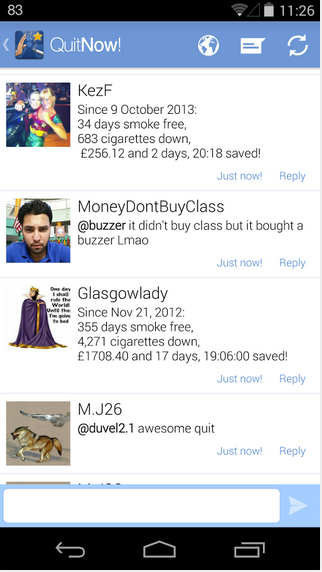
\includegraphics[width=.6\linewidth]{./images/application-quitnow-social}
  \captionof{figure}{QuitNow! networking~\citep{quitnow}}
  \label{application-quitnow-social}
\end{minipage}
\end{figure}

QuitNow!'s success can be measured through the feedback received through their Google Play store page, such as; \\

\indent\textbf{``Love it! I like that it resets the time if you slip and have a cigarette. It frustrated me to have to start over again, which I think helped me quit faster. Love the social part and the achievements you can earn. It's just great! Almost six months so far!''}~\citep{quitnow},\\and\\ 

\indent\textbf{``I love seeing how many cigarettes I've not smoked and the money I've saved. When I need an extra push the image galley is a nice reminder of why I'm quitting.''}~\citep{quitnow};\\

however some concerns are also raised in relation to the social networking aspect, evident by a users feedback of\\ 

\indent\textbf{``Too many people being racist or taking mick out of disabled people or just purely trolling quite bad when all peopld want Is support when quitting!!!''}~\citep{quitnow}, which will be addressed in section~\ref{sec:social-media}.

\newpage
\section{Techniques to Enhance User Engagement}\label{sec:techniques-to-enhance}
The following section will discuss some methods and techniques that can be used in order to increase user engagement with, and their satisfaction in the system.

\subsection{Rewards}\label{sec:rewards}
Rewards have been mentioned throughout section~\ref{sec:current-fields} as a means for motivation throughout all types of systems currently in operation today.
This section aims to divide the set of rewards into two subsets; being extrinsic and intrinsic~\citep{bread-and-games,fun-of-use,deci_extrinsic_2001,McGonigal:2011:RBW:1972527}, in order to obtain a better understanding of how rewards should be utilised in the systems we implement in future.

\subsubsection{Extrinsic}\label{sec:extrinsic}
Extrinsic rewards are those which are external to the user~\citep{deci_extrinsic_2001,McGonigal:2011:RBW:1972527} and can be rewards such as:
\begin{itemize}
	\item{Monetary,}
	\item{In-game currency~\citep{bread-and-games},}
	\item{Score~\citep{bread-and-games},}
	\item{Entries in a leader board~\citep{bread-and-games},}
	\item{Promotions,}
	\item{Leveling up~\citep{bread-and-games}, and}
	\item{Trophies}
\end{itemize}

\subsubsection{Intrinsic}\label{sec:intrinsic}
Intrinsic rewards are more personal to the user~\citep{patient-education-and-training}, some examples of intrinsic rewards are as follows:
\begin{itemize}
	\item{Enjoyment}
	\item{Challenge}
	\item{Excitement}
	\item{Education}
\end{itemize}

\subsubsection{Summary}
To summerise, rewards are an essential part of motivating a user to engage with a system; however care needs to be taken with what types of rewards are selected. It is important not to implement an unreasonable amount of extrinsic rewards as this can leave a user feeling bought and unaccomplished~\citep{openingSkinersBox,theSkinnerBox,McGonigal:2011:RBW:1972527,bread-and-games} sometimes making playing a game feel like doing work~\citep{turning-play-into-work}, instead extrinsic rewards should be added to complement intrinsic rewards and thus making them feel intrinsic as well. This all helps to create a system that increases satisfaction in the user, motivates a user to achieve higher goals within the system, provides higher productivity, and keeps the user feeling free and competent~\citep{intrinsic-motivation}.

\subsection{The Skinner Box}
The Skinner Box is a technique named by B.F. Skinner describing a small cage which houses a small animal, a lever and a way of delivering rewards to the animal~\citep{openingSkinersBox}. The idea was to train the animal to continuously hit the lever. The animal gets rewarded at random intervals for lever pressing, with the possibility of punishment if the lever is not pressed (usually by electric shock). This technique has been around since the 1930’s and has been implemented in video games since their inception~\citep{theSkinnerBox}.

\par
Game designers have expanded the Skinner Box concept and made it feel like second nature to players. They have done this by offering virtual rewards to players who achieve pre-defined goals (this is obvious in any games that have levels and/or virtual currency) and recently by punishing players for not playing regularly (usually by devaluing the players hard earned virtual currency or by making in-game possessions deteriorate).
 \par
The Skinner Box concept is a great way to develop players’ obsession to a game while offering no real world reward, instead just extrinsic rewards, often leaving the player wondering why they wasted so much time on the game~\citep{fiveCreepyWays,bread-and-games}. 

\subsection{Gamification}\label{sec:gamification}
Gamification is the process of integrating game dynamics and techniques into non-game processes. This is usually done to increase interaction, productivity or satisfaction.

\subsubsection{The History of Gamification}

\subsubsection{Elements in Game Design}
Gamification takes advantage of various features that are present in game design. The following paragraphs discuss the effectiveness of these features as well as the importance of their potential applications in enhancing user interactions beyond the gaming culture. 

\paragraph{\indent~Rewards.}
Rewards have already been discussed thoroughly in section~\ref{sec:rewards}, here we discuss how rewards are present in the gaming environment and how they can be used in other systems. 

\paragraph{\indent~Competition.}

\paragraph{\indent~Stories.}

\subsection{Virtual Reality}

\subsection{Effort Reduction}\label{sec:effort-reduction}

\subsection{Usability}

\subsection{Social Media}\label{sec:social-media}

\subsection{Education}

\subsection{Summary}
In order for a system to be motivating; it should offer some kind of intrinsic reward to the user, which is easier to implement if the system already has a meaning purpose that would interest the user on its own; such as: a system that aims to educate, a system that assists a worker in their job, or a system that assists a user to do their day-to-day tasks.

\par
A system should be interesting, in order to do this new content should be added regularly. The system needs a point i.e. the system shouldn't be designed with the main aim of encouraging users to use it, because if the user doesn't get anything out of it then there is not reason for the user to interact with the system. 
In addition to the point of the system, it is important to have enough interesting content so the user is not constantly thinking about what they are trying to achieve. There is a delicate balance here between being to the point and being distracting.

\par
The system must not be difficult to use, users should not need to learn a new technology or interface to interact with the system. 37\% of Australians have a smartphone, with countries such as Singapore showing a penetration of 62\%~\citep{smartphone-use-in-au}, this provides a basic tool to be utilising in these systems.

\par
Humans have a natural desire to compete~\citep{bread-and-games}, this can be leveraged in the systems we design through tools such as; leader boards, and achievements, in order to make a system naturally motivating.
Social media in a great way to advertise these achievements to bring the competition to a grander scale; however care should be taken to avoid slanderous comments from non-constructive individuals, usually taken care of by giving the user control over who can see their updates.

\newpage
\section{City Evolutions}
\subsection{Analysis}
Analyse the current setup of the city evolutions project.\\
discuss the current statistics:
\begin{itemize}
	\item{Good points (project clearly had a boost on open)}
	\item{Bad points (users aren't motivated to keep coming back and scanning the qr code because there isnt a lot of new material)}
\end{itemize}

\begin{figure}[ht!]
	\centering
	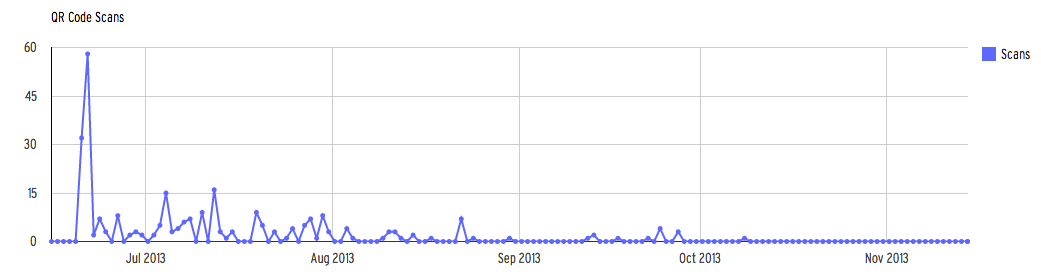
\includegraphics[width=150mm]{./images/OverallQRCodeDownload}
	\caption{QR Code - Overall scans}
	\label{QR-overall-access-overTime}
\end{figure}

\begin{figure}[ht!]
	\centering
	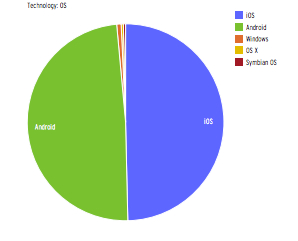
\includegraphics[width=50mm]{./images/OSAccess}
	\caption{QR Code - OS spread}
	\label{QR-OS-access}
\end{figure}

\begin{figure}[ht!]
	\centering
	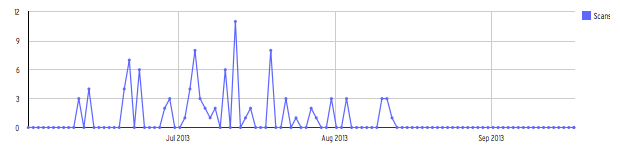
\includegraphics[width=150mm]{./images/threkeld-scans}
	\caption{QR Code - Threlkeld Speak scans}
	\label{QR-threkeld}
\end{figure}

\begin{figure}[ht!]
	\centering
	
\includegraphics[width=50mm]{./images/qrcode-threlkeld}
	\caption{QR Code - Threlkeld Speak}
	\label{QR-threkeld-barcode}
\end{figure}

\begin{table}
	\centering
	\begin{tabular}{|c|c|c|}\hline
		\textbf{Application} & 	\textbf{Number of Scans} & \textbf{Interactivity (see table~\ref{table:interactivity-description})} \\\hline
		Macquaries Chest & 2 & Low\\
		Car Culture & 3 & None\\
		Lansescape & 34 & Medium\\
		Coal Collector & 36 & Medium\\
		Dreaming & 3 & None\\
		Settling In & 28 & Low\\
		Major Morisset & 36 & Low\\
		Evolutions & 6 & None\\
		Shanghai & 2 & Medium\\
		Boom \& Bust & 2 & Low\\
		Threlkeld 	&	132 & Medium\\\hline
	\end{tabular}
	\caption{City Evolutions Applications and their popularity}
	\label{table:application-popularity}
\end{table}

\begin{table}
	\centering
	\bgroup
	\def\arraystretch{2.5}%  1 is the default, change whatever you need
	\begin{tabular}{|l|l|}\hline
		\textbf{Level} 	& \textbf{Description}\\\hline
		None 	& \pbox{20cm}{No user input is taken at all, generally a slideshow or movie} \\\hline
		Low 	& \pbox{20cm}{Generally a single has basic control over the application\\ 
				  			  i.e. User makes movement to trigger the application to take action.} \\\hline
		Medium 	& \pbox{20cm}{Users have basic control over the application and are given constant\\
							  feedback, the more users the more feedback is received.}\\\hline
		High 	& \pbox{20cm}{Users have fine grained control over the application,\\ 
							  with constant feedback and a reason to come back to the application\\
							  i.e. scores are saved, competitions are run, etc.}\\\hline
	\end{tabular}
	\egroup
	\caption{Description of interactivity levels used in \ref{table:application-popularity}}
	\label{table:interactivity-description}
\end{table}

\newpage
\subsection{Proposal}

\begin{figure}
\centering
\begin{minipage}{.5\textwidth}
  \centering
  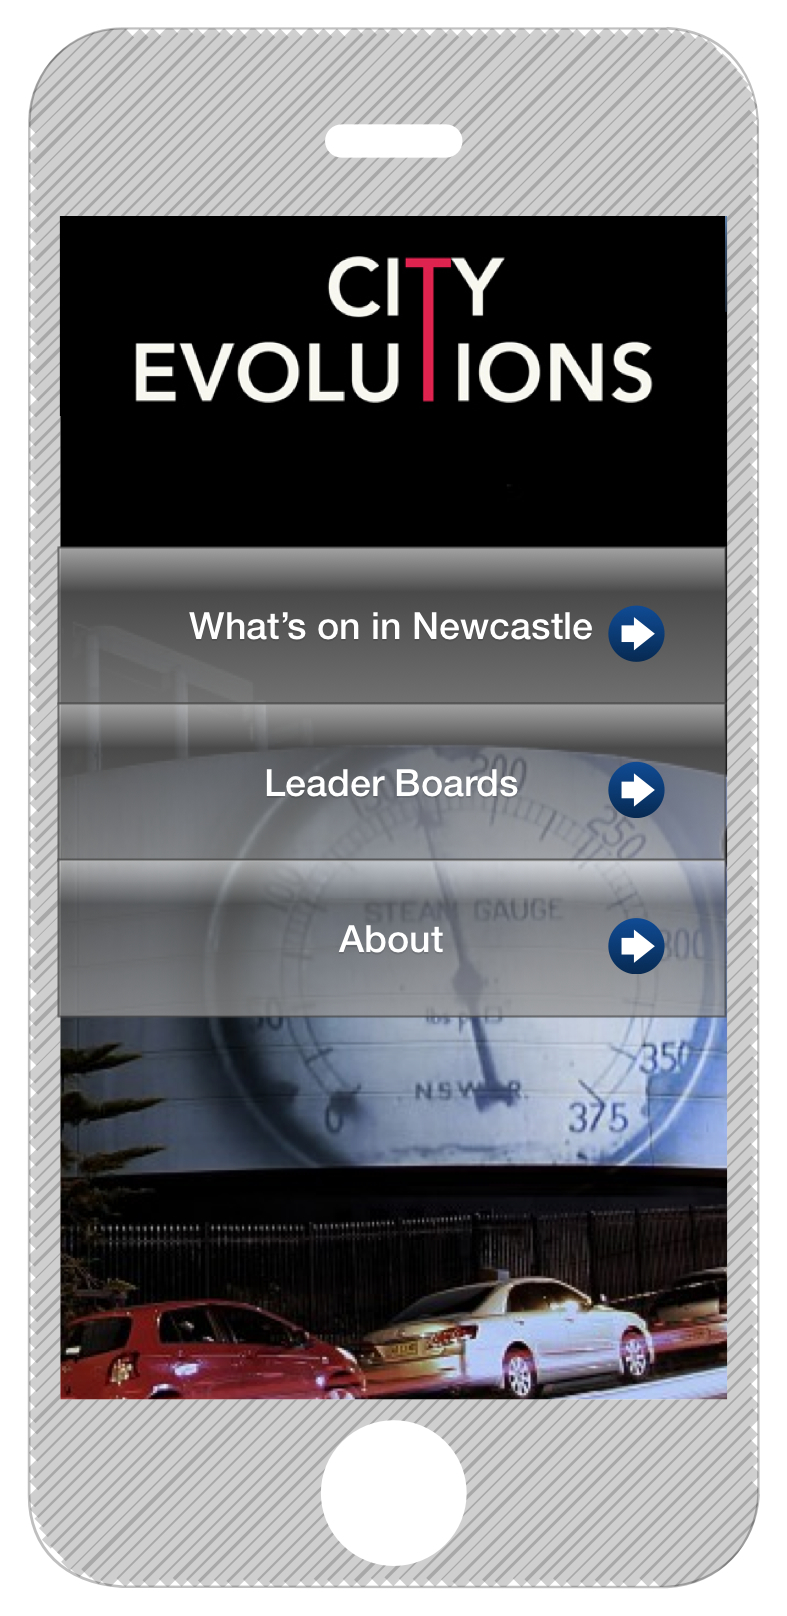
\includegraphics[width=.6\linewidth]{./images/iphone-interface}
  \captionof{figure}{Application start screen}
  \label{iphone-interface-startscreen}
\end{minipage}%
\begin{minipage}{.5\textwidth}
  \centering
  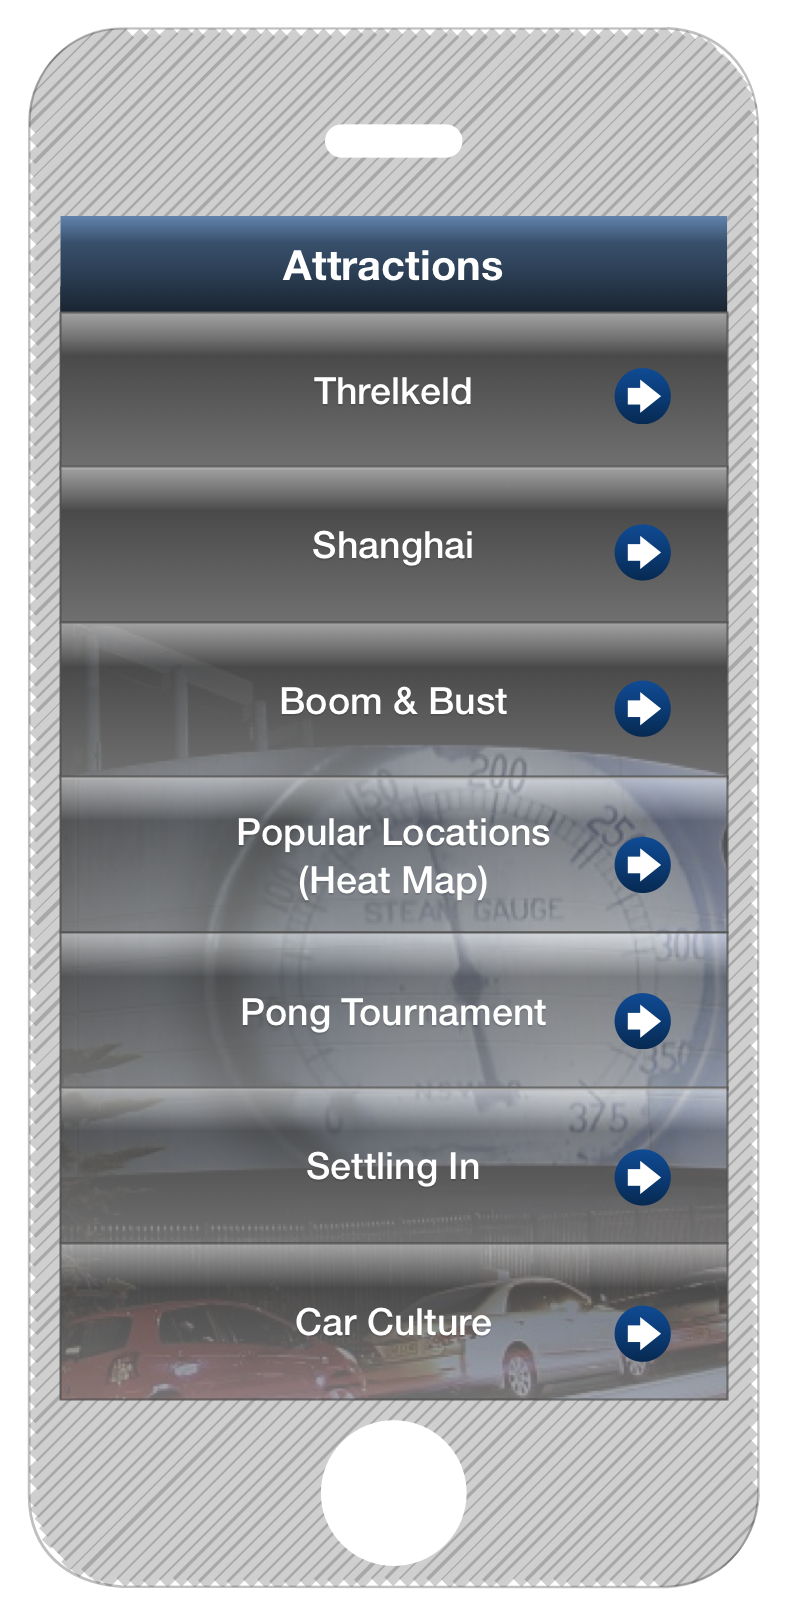
\includegraphics[width=.6\linewidth]{./images/iphone-interface-menu}
  \captionof{figure}{Application Menu}
  \label{iphone-interface-menu}
\end{minipage}
\end{figure}


\begin{figure}
\centering
\begin{minipage}{.5\textwidth}
  \centering
  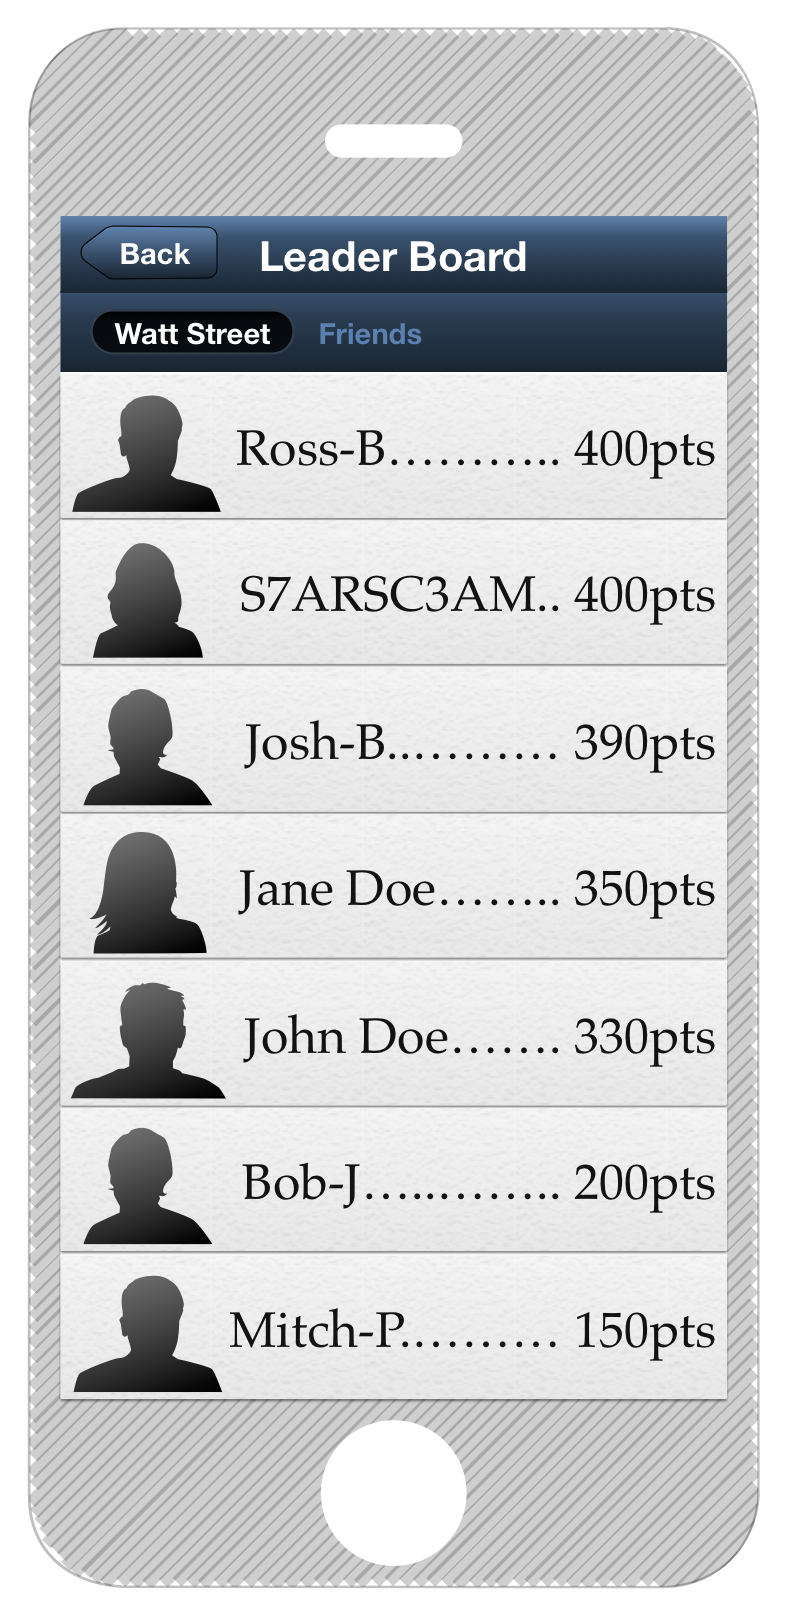
\includegraphics[width=.6\linewidth]{./images/iphone-interface-leaderboard}
  \captionof{figure}{Application leader board}
  \label{iphone-interface-leaderboard}
\end{minipage}%
\begin{minipage}{.5\textwidth}
  \centering
  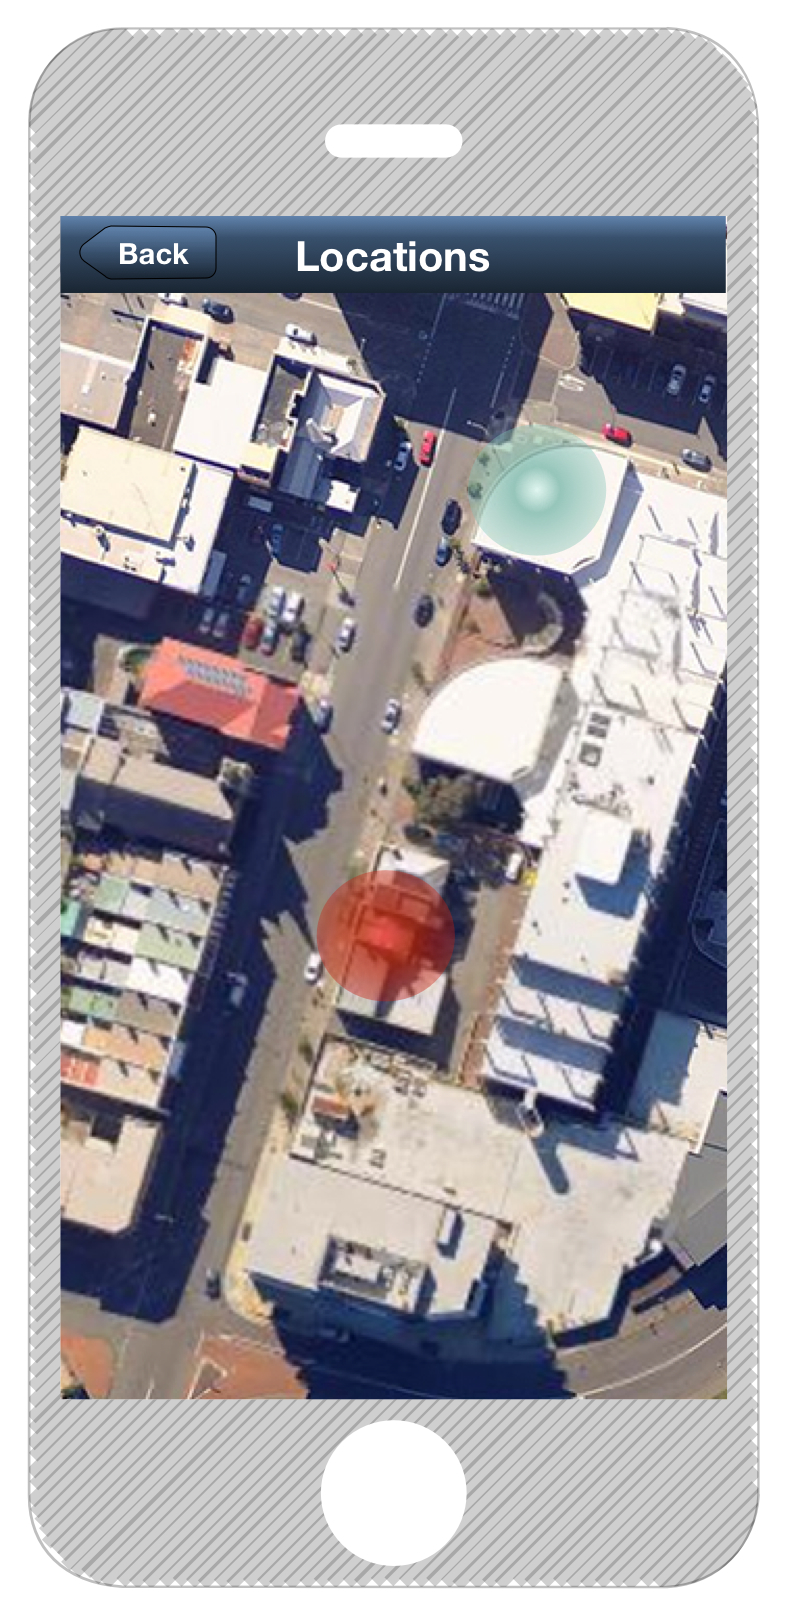
\includegraphics[width=.6\linewidth]{./images/iphone-interface-map}
  \captionof{figure}{Application locations map}
  \label{iphone-interface-map}
\end{minipage}
\end{figure}

\begin{figure}[ht!]
	\centering
	\includegraphics[width=125mm]{./images/MultiPlayerChurchGame}
	\caption{Multiplayer pong-style game to be played at the church.}
	\label{application-multiPlyerPong}
\end{figure}

\newpage
\section{Discussion}
%
Give an extended and detailed discussion of your study. explain what we can learn from your study.
%

\section{Conclusion}
%
A brief final summary of the main achievements and outcomes. Possibly some suggestions for future work that can follow on from your project.%


\section{Glossary}
%
\subsection*{Acknowledgements}
The author is grateful to ....
%
\vskip 0.2in
\newpage
\bibliographystyle{apalike}
\bibliography{./literature.bib}


\end{document}
